\chapter{Tecnologias Utilizadas}
Considerando os aspectos discutidos no capítulo 2 sobre possíveis e impossíveis instrumentos para o nosso contexto, por fim foram selecionadas as tecnologias que serão efetivamente utilizados no projeto, as quais são descritas neste capítulo.

\section{Dispositivo Embarcado}
Partindo disso, selecionou-se a plataforma de desenvolvimento do Sensor Tag da Texas Instruments como componente embarcado de cada macaco. Trata-se de uma placa leve que contém 6 sensores, incluindo de temperatura, e comunicador BLE. Seu datasheet pode ser encontrado nas referências deste trabalho.

\begin{figure}[ht]
  \centering
    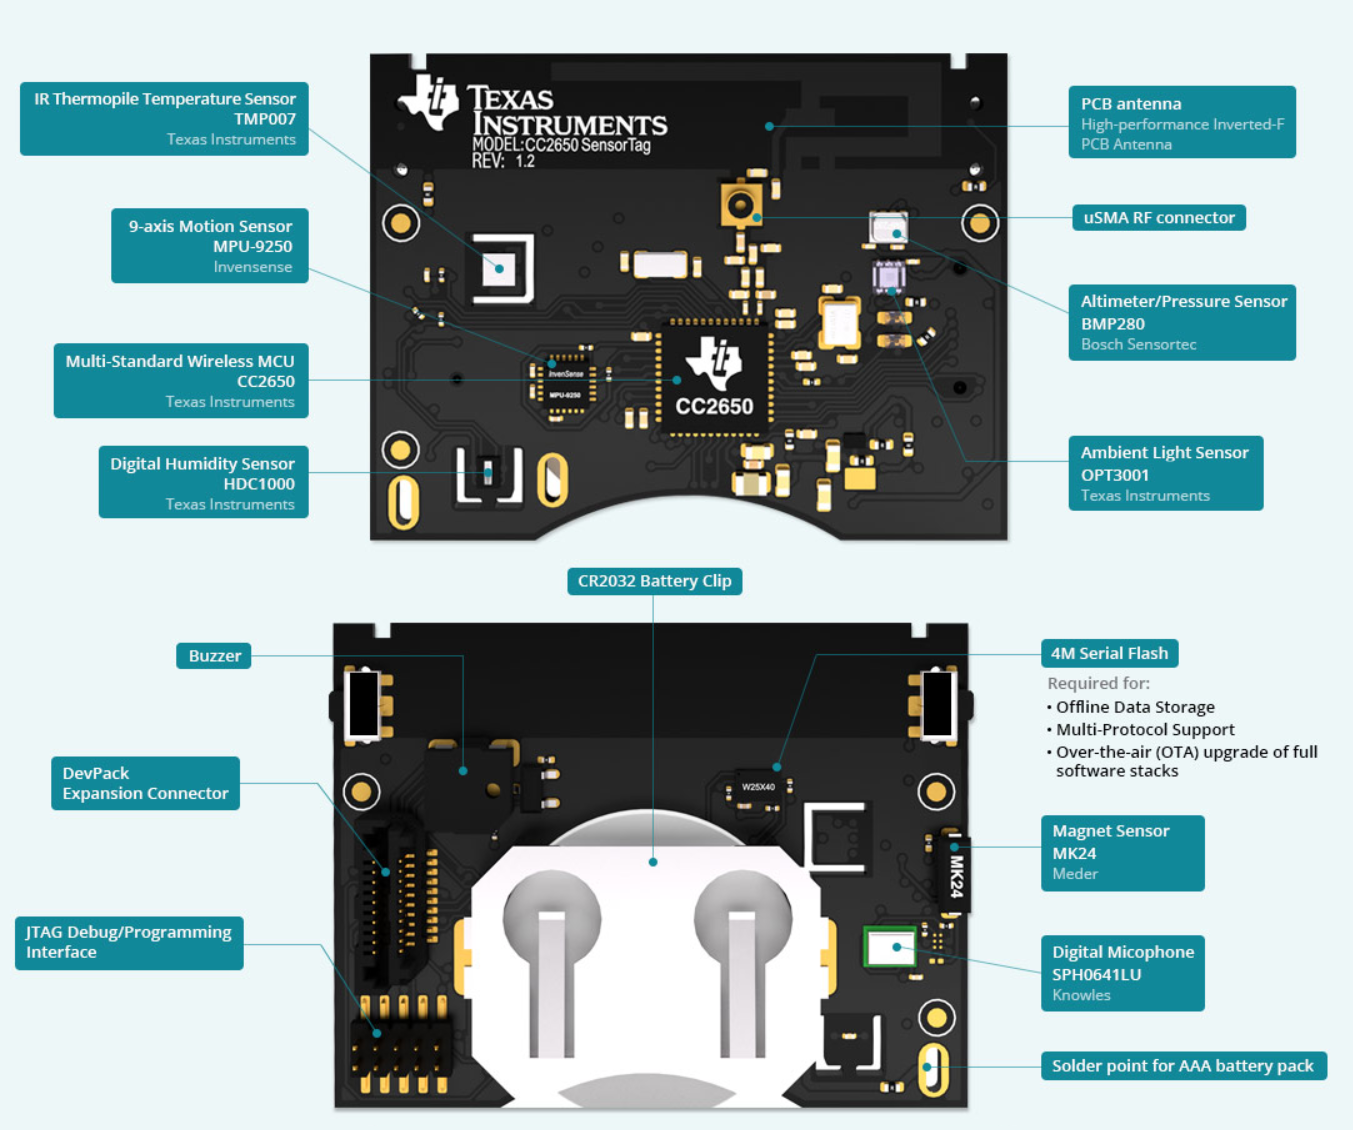
\includegraphics[scale=0.5]{sensortag}
  \caption{Componentes do Sensor Tag (Fonte: extraído do site da Texas Instruments)}
\end{figure}

Foi utilizado um Raspberry Pi 2 para receber por BLE os dados de cada Sensor Tag e enviá-los por Wi-fi para o servidor, que pode ser local ou em nuvem. 

\section{Servidor}
Foi escolhido o banco de dados relacional MySQL da Oracle por se tratar de um sistema open source simples, embora completo.

O projeto SIMIOS prevê o rastreio de animais em reservas, o que envolve, como visto anteriormente, no máximo cerca de 50 animais em grandes reservas. Dessa forma, sabemos que não envolve sobrecarga de acessos por segundo e mesmo isto poderia ser corrigido com buffering.

Um ponto negativo do MySQL é que sua escalabilidade pode ser prejudicada - cada servidor tem um tamanho limitado e cada set de dados só pode ser alocado em um servidor (não suporta particionamento), o que pode ser prejudicial em casos que deseja-se guardar no banco grande quantidade de dados. Para corrigir tal empecilho é possível implementar importação de dados.

\section{Software}
Para desenvolvimento do programa computacional que é executado no servidor, foi escolhida a linguagem de programação Java, com suporte de frameworks Spring e JPA, facilitando principalmente os processos de queries do banco de dados, de autenticação e autorização e de mapeamento de interface model-view-controller (MVC).

Por se tratar de uma aplicação de histórico de dados, pouquíssimo processamento está previsto e a computação pode ser realizada em tempo real pelo computador do usuário. Dessa forma, não se faz necessário o uso de linguagem de programação de execução eficiente (C++, por exemplo).
